%%%%%%%%%%%%%%%%%%%%%%
% Overleaf (WriteLaTeX) Example: Molecular Chemistry Presentation
%
% Source: http://www.overleaf.com
%
% In these slides we show how Overleaf can be used with standard 
% chemistry packages to easily create professional presentations.
% 
% Feel free to distribute this example, but please keep the referral
% to overleaf.com
%%%%%%%%%%%%%%%%%%%%%%%%%%%%%%%%%%%%%%%%%%%%%%%%%%%%%%%%%%%%%%%%%%%%%%

\documentclass[dvipsnames]{beamer}

% For more themes, color themes and font themes, see:
% http://deic.uab.es/~iblanes/beamer_gallery/index_by_theme.html
%
\mode<presentation>
{
  \usetheme{CambridgeUS}       % or try default, Darmstadt, Warsaw, ...
  \usecolortheme{orchid} % or try albatross, beaver, crane, ...
  \usefonttheme{serif}    % or try default, structurebold, ...
  \setbeamertemplate{navigation symbols}{}
  \setbeamertemplate{caption}[numbered]
} 

\usepackage[english]{babel}
\usepackage[utf8x]{inputenc}
\usepackage[mmddyyyy]{datetime}
\usepackage{hyperref}
\usepackage{graphicx}
\usepackage{caption}
\usepackage{comment}
\usepackage{amsmath}
\usepackage{soul} % For strikethroughs
\usepackage{mathtools}
\DeclarePairedDelimiter{\ceil}{\lceil}{\rceil}
\DeclarePairedDelimiter{\floor}{\lfloor}{\rfloor}
\newcommand\oversetsymb[2]{\stackrel{\mathclap{\normalfont\mbox{#1}}}{#2}}
\newcommand\myoutlineslide{
	\begin{frame}{Outline}
		\tableofcontents
	\end{frame}
}
\usepackage{marvosym}
\usepackage{chngcntr}
\counterwithin*{equation}{section}
\counterwithin*{equation}{subsection}
%\usepackage{enumitem}
\usepackage{nicefrac}
% \useoutertheme{infolines}

% Theorems, propositions, lemmas...
\newtheorem{thm}{Theorem}[section]
\newtheorem{prop}[thm]{Proposition}
\newtheorem{lem}[thm]{Lemma}
\newtheorem{cor}[thm]{Corollary}
\newtheorem{defn}[thm]{Definition}
\newtheorem{rem}[thm]{Remark}

%
\usepackage{tikz}
\usetikzlibrary{arrows,shapes,trees, backgrounds}

% On Overleaf, these lines give you sharper preview images.
% You might want to `comment them out before you export, though.
%\usepackage{pgfpages}
%\pgfpagesuselayout{resize to}[%
 % physical paper width=8in, physical paper height=6in]

\AtBeginSection[]{
  \begin{frame}
  \vfill
  \centering
  \begin{beamercolorbox}[sep=8pt,center,shadow=true,rounded=true]{title}
    \usebeamerfont{title}\insertsectionhead\par%
  \end{beamercolorbox}
  \vfill
  \end{frame}
}

\AtBeginSubsection[]{
  \begin{frame}
  \vfill
  \centering
  \begin{beamercolorbox}[sep=8pt,center,shadow=true,rounded=true]{title}
    \usebeamerfont{title}\insertsubsectionhead\par%
  \end{beamercolorbox}
  \vfill
  \end{frame}
}

\AtBeginSubsubsection[]{
  \begin{frame}
  \vfill
  \centering
  \begin{beamercolorbox}[sep=8pt,center,shadow=true,rounded=true]{title}
    \usebeamerfont{title}\insertsubsubsectionhead\par%
  \end{beamercolorbox}
  \vfill
  \end{frame}
}

%\renewcommand{\bf}[1]{\textbf{#1}}
\newcommand{\shortsim}{\raise.17ex\hbox{$\scriptstyle \sim$}}
\newcommand{\True}{\emph{True}\ }
\newcommand{\False}{\emph{False}\ }
\newcommand{\T}{\emph{\textbf{T}}\ }
\newcommand{\F}{\emph{\textbf{F}}\ }
\newcommand{\TODO}{\textcolor{red}{\bf{TODO}}\ }
\newcommand{\ifftext}{\bf{iff}}
\renewcommand{\neg}{\shortsim}
\newcommand{\?}{\textcolor{red}{\textbf{?}}}
\newcommand{\correct}[1]{\textcolor{green}{\textbf{#1}}}
\newcommand{\pwset}[1]{\mathcal{P}(\lbrace #1 \rbrace)}

% Card voting
\newcommand{\twocards}[2]{
	\begin{figure}
		\centering
		\begin{tabular}{cc}
			\centering
			\tikz \node[draw,fill=green!50] {#1}; &
             \tikz \node[draw,fill=cyan] {#2}; 
		\end{tabular}	
	\end{figure}
}

\newcommand{\threecards}[3]{
	\begin{figure}
		\centering
		\begin{tabular}{ccc}
			\centering
			\tikz \node[draw,fill=green!50] {#1}; &
             \tikz \node[draw,fill=cyan] {#2}; &
             \tikz \node[draw,fill=yellow] {#3}; 
		\end{tabular}	
	\end{figure}
}

\newcommand{\fourcards}[4]{
	\begin{figure}
		\centering
		\begin{tabular}{cccc}
			\centering
			\tikz \node[draw,fill=green!50] {#1}; &
             \tikz \node[draw,fill=cyan] {#2}; & 
            \tikz \node[draw,fill=yellow] {#3}; & 
            \tikz \node[draw,fill=white] {#4};
		\end{tabular}	
	\end{figure}
}
% Here's where the presentation starts, with the info for the title 
% slide
\title[The Pigeonhole Principle]{Pigeonhole Principle}
\author{\empty}
\institute{CMSC250}

%\newdate{shortlecdate}{22}{06}{2016}
%\renewcommand{\dateseparator}{-}
%\date{\displaydate{shortlecdate}}
\setbeamertemplate{caption}{\raggedright\insertcaption\par} % To avoid "Figure 1:" before "Look."

\date{\empty}

\begin{document}
\maketitle
%\myoutlineslide

\begin{frame}{Look at these pigeons.}
\begin{figure}
	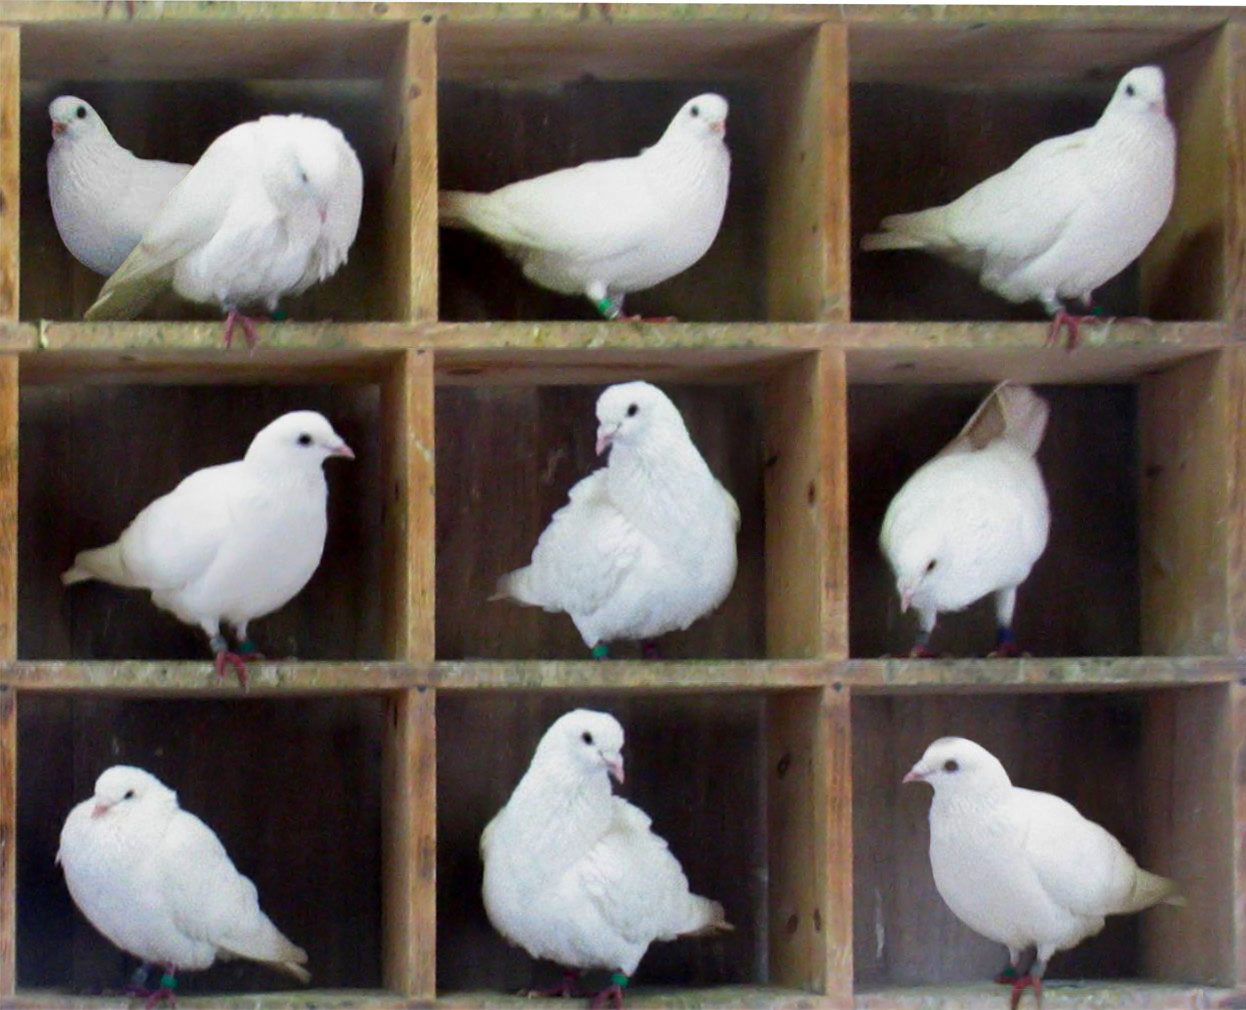
\includegraphics[scale=.17]{img/TooManyPigeons}
	\caption{Look.}
	\label{fig:pigeons}
\end{figure}
\end{frame}

\begin{frame}{Examples first}
\begin{enumerate}
	\item Is there a pair of you with the same birthday month? \pause \textcolor{red}{Yes, since there are more than 12 of you!}
	\item Is there a pair of you with the same birthday week?\pause \textcolor{red}{Yes, since there are more than 52 of you!}
	\item Is there a pair of New Yorkers with the same number of hairs on their heads? \pause \textcolor{red}{Yes! Number of hairs on your head $\leq  300,000$, New Yorkers $\geq 8,000,000$.}
\end{enumerate}

\end{frame}

\begin{frame}{Examples first}
	\begin{enumerate}
	  \setcounter{enumi}{3}
		\item Let $A = \lbrace 1, 2, 3, 4, 5, 6,  7, 8 \rbrace$. If I pick 5 integers, is it the case that at least one pair of integers has a sum of $9$? \pause \textcolor{red}{Yes. Pigeonholes = pairs of ints that sum to 9: \begin{align*} 
								 (1, 8) \\ 
								(2, 7)\\  
								(3, 6) \\ 
								(4, 5)  
						\end{align*} 
			and pigeons = ints to pick.}
		\end{enumerate}
\end{frame}
\begin{frame}{Examples first}
	\begin{enumerate}
			  \setcounter{enumi}{4}
		\item  Let $A \subseteq \{ 1, 2, \dots , 10 \}$, and $\vert A \vert = 6$. Is there a pair of subsets of $A$ that have the same sum? \pause \textcolor{red}{Yes. \\There are $2^6 = 64$ subsets of $A$. Max sum: $10+9+\dots + 5 = 45$ \\ Min sum: $0$ \\ $46$ different sums (pigeonholes) \\ $64$ different subsets (pigeons).} 
		\end{enumerate}
\end{frame}

\begin{frame}{Examples first}
	\begin{enumerate}
				  \setcounter{enumi}{5}
		\item  Is it true that within a group of 700 people, there must be 2 who have the same \textbf{first} and \textbf{last} initials? \pause \textcolor{red}{Yes. \\ There are $26^2 = 676$ different sets of first and last initials (pigeonholes) \\ There are  700 people (pigeons).}
		\end{enumerate}
\end{frame}

\begin{frame}{Formal Statement of the principle}

\begin{block}{Pigeonhole Principle}
Let $m, n \in \mathbb{N}^{\geq 1}$. If $n$ pigeons fly into $m$ pigeonholes and $n > m$, then \textbf{at least one} pigeonhole will contain more than one pigeon.
\end{block} \pause
\begin{itemize}
	\item \textcolor{red}{Can I have empty pigeonholes?} \twocards{Yes}{No} \pause \textbf{Absolutely}. Only thing we need is one pigeonhole with at least 2 pigeons. 
	\item Example: There might not be somebody with initials $(X,Y)$.
\end{itemize}

\begin{block}{Pigeonhole Principle (in functions)}
Let $A$ and $B$ be finite sets such that $\vert A \vert > \vert B \vert$. Then, there does not exist a one-to-one function $f:A \mapsto B$.
\end{block}
\end{frame}

\begin{frame}{Some more advanced examples}
\begin{enumerate} \small
	\item If there are $105$ of you, do at least \textbf{9} of you have the same birthday month? \pause  \textcolor{red}{Yes. If there are at most 8, then $ 8\times 12 = 96 < 105$, but $9 \times 12 =108 > 105$ }
	\item If there are 105 of you, are there at least \textbf{3} of you with the same birthday week? \pause \textcolor{red}{Yes. If there are at most 2, then $2\times 52 = 104 < 105$} 
		\item Is it true that within a group of 86 people, there exist \textbf{at least 4} with the same \textbf{last initial} (e.g \textbf{B} for Justin \textbf{B}ieber). \pause \textcolor{red}{Yes. Pigeonholes = \#{}initials=$26$. For $k=3$, $86 > 3 \times 26 = 78$} 
\end{enumerate}
\end{frame}

\begin{frame}{Another interesting example}
\begin{enumerate}
	\setcounter{enumi}{3}
	\item   Let $M=\{1, 2, 3, \dots, 1000\}$ and suppose $A \subseteq M$ such that $\vert A \vert = 20$. How many \textbf{subsets of} $\mathbf{A}$ sum to the same number? \pause \textcolor{red}{There are $2^{20}$ subsets of $A$. The max sum is $1000 + 999 + \dots + 981 = \displaystyle\sum_{i=1}^{1000} i - \displaystyle\sum_{i=1}^{980} i \overset{\text{Gauss}}{{=\joinrel=}} \frac{1000 \cdot 1001}{2} - \frac{980 \cdot 981}{2} = 19810$. The min sum is 0, corresponding to $\emptyset \subseteq A$. So $19811$ sums. Since $\lceil \nicefrac{2^{20}}{19811}\rceil = 53$ (yes, you may totally use a calculator here), there are 53 subsets of $A$ that sum to the same number.} \pause
	\item What kind of proof is this? 
\end{enumerate}
\vspace{-.50in}
\hspace{-.6in} \fourcards{By cases}{Non-constructive}{By contradiction}{Something Else} \pause
\textcolor{blue}{Non-constructive! It proves that it's a \textbf{logical necessity} that $53$ subsets map to the same sum, but doesn't tell you \textbf{anything} (e.g cardinality) of the subsets.}

\end{frame}

\begin{frame}{Generalization}
\begin{block}{Generalized Pigeonhole Principle}
Let $n$ and $m$ be positive integers. Then, if there exists a positive integer $k$ such that $n > km$ and $n$ pigeons fly into $m$ pigeonholes, there will be \textbf{at least one} pigeonhole with \textbf{at least $k + 1$} pigeons.
\end{block} 

\begin{itemize}
	\item Our second example set consisted of examples of the \textbf{generalized} form of the principle.
\end{itemize}
\end{frame}


\end{document}